\documentclass[1p]{elsarticle_modified}
%\bibliographystyle{elsarticle-num}

%\usepackage[colorlinks]{hyperref}
%\usepackage{abbrmath_seonhwa} %\Abb, \Ascr, \Acal ,\Abf, \Afrak
\usepackage{amsfonts}
\usepackage{amssymb}
\usepackage{amsmath}
\usepackage{amsthm}
\usepackage{scalefnt}
\usepackage{amsbsy}
\usepackage{kotex}
\usepackage{caption}
\usepackage{subfig}
\usepackage{color}
\usepackage{graphicx}
\usepackage{xcolor} %% white, black, red, green, blue, cyan, magenta, yellow
\usepackage{float}
\usepackage{setspace}
\usepackage{hyperref}

\usepackage{tikz}
\usetikzlibrary{arrows}

\usepackage{multirow}
\usepackage{array} % fixed length table
\usepackage{hhline}

%%%%%%%%%%%%%%%%%%%%%
\makeatletter
\renewcommand*\env@matrix[1][\arraystretch]{%
	\edef\arraystretch{#1}%
	\hskip -\arraycolsep
	\let\@ifnextchar\new@ifnextchar
	\array{*\c@MaxMatrixCols c}}
\makeatother %https://tex.stackexchange.com/questions/14071/how-can-i-increase-the-line-spacing-in-a-matrix
%%%%%%%%%%%%%%%

\usepackage[normalem]{ulem}

\newcommand{\msout}[1]{\ifmmode\text{\sout{\ensuremath{#1}}}\else\sout{#1}\fi}
%SOURCE: \msout is \stkout macro in https://tex.stackexchange.com/questions/20609/strikeout-in-math-mode

\newcommand{\cancel}[1]{
	\ifmmode
	{\color{red}\msout{#1}}
	\else
	{\color{red}\sout{#1}}
	\fi
}

\newcommand{\add}[1]{
	{\color{blue}\uwave{#1}}
}

\newcommand{\replace}[2]{
	\ifmmode
	{\color{red}\msout{#1}}{\color{blue}\uwave{#2}}
	\else
	{\color{red}\sout{#1}}{\color{blue}\uwave{#2}}
	\fi
}

\newcommand{\Sol}{\mathcal{S}} %segment
\newcommand{\D}{D} %diagram
\newcommand{\A}{\mathcal{A}} %arc


%%%%%%%%%%%%%%%%%%%%%%%%%%%%%5 test

\def\sl{\operatorname{\textup{SL}}(2,\Cbb)}
\def\psl{\operatorname{\textup{PSL}}(2,\Cbb)}
\def\quan{\mkern 1mu \triangleright \mkern 1mu}

\theoremstyle{definition}
\newtheorem{thm}{Theorem}[section]
\newtheorem{prop}[thm]{Proposition}
\newtheorem{lem}[thm]{Lemma}
\newtheorem{ques}[thm]{Question}
\newtheorem{cor}[thm]{Corollary}
\newtheorem{defn}[thm]{Definition}
\newtheorem{exam}[thm]{Example}
\newtheorem{rmk}[thm]{Remark}
\newtheorem{alg}[thm]{Algorithm}

\newcommand{\I}{\sqrt{-1}}
\begin{document}

%\begin{frontmatter}
%
%\title{Boundary parabolic representations of knots up to 8 crossings}
%
%%% Group authors per affiliation:
%\author{Yunhi Cho} 
%\address{Department of Mathematics, University of Seoul, Seoul, Korea}
%\ead{yhcho@uos.ac.kr}
%
%
%\author{Seonhwa Kim} %\fnref{s_kim}}
%\address{Center for Geometry and Physics, Institute for Basic Science, Pohang, 37673, Korea}
%\ead{ryeona17@ibs.re.kr}
%
%\author{Hyuk Kim}
%\address{Department of Mathematical Sciences, Seoul National University, Seoul 08826, Korea}
%\ead{hyukkim@snu.ac.kr}
%
%\author{Seokbeom Yoon}
%\address{Department of Mathematical Sciences, Seoul National University, Seoul, 08826,  Korea}
%\ead{sbyoon15@snu.ac.kr}
%
%\begin{abstract}
%We find all boundary parabolic representation of knots up to 8 crossings.
%
%\end{abstract}
%\begin{keyword}
%    \MSC[2010] 57M25 
%\end{keyword}
%
%\end{frontmatter}

%\linenumbers
%\tableofcontents
%
\newcommand\colored[1]{\textcolor{white}{\rule[-0.35ex]{0.8em}{1.4ex}}\kern-0.8em\color{red} #1}%
%\newcommand\colored[1]{\textcolor{white}{ #1}\kern-2.17ex	\textcolor{white}{ #1}\kern-1.81ex	\textcolor{white}{ #1}\kern-2.15ex\color{red}#1	}

{\Large $\underline{12n_{0581}~(K12n_{0581})}$}

\setlength{\tabcolsep}{10pt}
\renewcommand{\arraystretch}{1.6}
\vspace{1cm}\begin{tabular}{m{100pt}>{\centering\arraybackslash}m{274pt}}
\multirow{5}{120pt}{
	\centering
	\includegraphics[width=112pt]{../../../GIT/diagram.site/Diagrams/png/2670_12n_0581.png}\\
\ \ \ A knot diagram\footnotemark}&
\allowdisplaybreaks
\textbf{Linearized knot diagam} \\
\cline{2-2}
 &
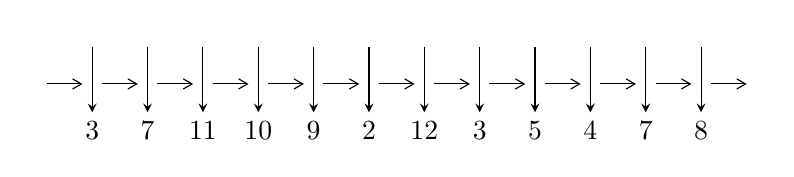
\begin{tikzpicture}[x=20pt, y=17pt]
	% nodes
	\node (C0) at (0, 0) {};
	\node (C1) at (1, 0) {};
	\node (C1U) at (1, +1) {};
	\node (C1D) at (1, -1) {3};

	\node (C2) at (2, 0) {};
	\node (C2U) at (2, +1) {};
	\node (C2D) at (2, -1) {7};

	\node (C3) at (3, 0) {};
	\node (C3U) at (3, +1) {};
	\node (C3D) at (3, -1) {11};

	\node (C4) at (4, 0) {};
	\node (C4U) at (4, +1) {};
	\node (C4D) at (4, -1) {10};

	\node (C5) at (5, 0) {};
	\node (C5U) at (5, +1) {};
	\node (C5D) at (5, -1) {9};

	\node (C6) at (6, 0) {};
	\node (C6U) at (6, +1) {};
	\node (C6D) at (6, -1) {2};

	\node (C7) at (7, 0) {};
	\node (C7U) at (7, +1) {};
	\node (C7D) at (7, -1) {12};

	\node (C8) at (8, 0) {};
	\node (C8U) at (8, +1) {};
	\node (C8D) at (8, -1) {3};

	\node (C9) at (9, 0) {};
	\node (C9U) at (9, +1) {};
	\node (C9D) at (9, -1) {5};

	\node (C10) at (10, 0) {};
	\node (C10U) at (10, +1) {};
	\node (C10D) at (10, -1) {4};

	\node (C11) at (11, 0) {};
	\node (C11U) at (11, +1) {};
	\node (C11D) at (11, -1) {7};

	\node (C12) at (12, 0) {};
	\node (C12U) at (12, +1) {};
	\node (C12D) at (12, -1) {8};
	\node (C13) at (13, 0) {};

	% arrows
	\draw[->,>={angle 60}]
	(C0) edge (C1) (C1) edge (C2) (C2) edge (C3) (C3) edge (C4) (C4) edge (C5) (C5) edge (C6) (C6) edge (C7) (C7) edge (C8) (C8) edge (C9) (C9) edge (C10) (C10) edge (C11) (C11) edge (C12) (C12) edge (C13) ;	\draw[->,>=stealth]
	(C1U) edge (C1D) (C2U) edge (C2D) (C3U) edge (C3D) (C4U) edge (C4D) (C5U) edge (C5D) (C6U) edge (C6D) (C7U) edge (C7D) (C8U) edge (C8D) (C9U) edge (C9D) (C10U) edge (C10D) (C11U) edge (C11D) (C12U) edge (C12D) ;
	\end{tikzpicture} \\
\hhline{~~} \\& 
\textbf{Solving Sequence} \\ \cline{2-2} 
 &
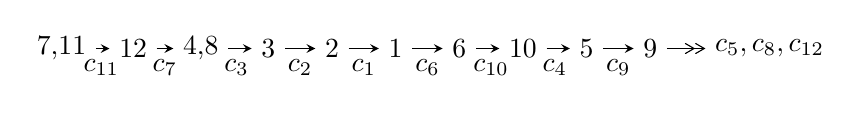
\begin{tikzpicture}[x=23pt, y=7pt]
	% node
	\node (A0) at (-1/8, 0) {7,11};
	\node (A1) at (1, 0) {12};
	\node (A2) at (33/16, 0) {4,8};
	\node (A3) at (25/8, 0) {3};
	\node (A4) at (33/8, 0) {2};
	\node (A5) at (41/8, 0) {1};
	\node (A6) at (49/8, 0) {6};
	\node (A7) at (57/8, 0) {10};
	\node (A8) at (65/8, 0) {5};
	\node (A9) at (73/8, 0) {9};
	\node (C1) at (1/2, -1) {$c_{11}$};
	\node (C2) at (3/2, -1) {$c_{7}$};
	\node (C3) at (21/8, -1) {$c_{3}$};
	\node (C4) at (29/8, -1) {$c_{2}$};
	\node (C5) at (37/8, -1) {$c_{1}$};
	\node (C6) at (45/8, -1) {$c_{6}$};
	\node (C7) at (53/8, -1) {$c_{10}$};
	\node (C8) at (61/8, -1) {$c_{4}$};
	\node (C9) at (69/8, -1) {$c_{9}$};
	\node (A10) at (11, 0) {$c_{5},c_{8},c_{12}$};

	% edge
	\draw[->,>=stealth]	
	(A0) edge (A1) (A1) edge (A2) (A2) edge (A3) (A3) edge (A4) (A4) edge (A5) (A5) edge (A6) (A6) edge (A7) (A7) edge (A8) (A8) edge (A9) ;
	\draw[->>,>={angle 60}]	
	(A9) edge (A10);
\end{tikzpicture} \\ 

\end{tabular} \\

\footnotetext{
The image of knot diagram is generated by the software ``\textbf{Draw programme}" developed by Andrew Bartholomew(\url{http://www.layer8.co.uk/maths/draw/index.htm\#Running-draw}), where we modified some parts for our purpose(\url{https://github.com/CATsTAILs/LinksPainter}).
}\phantom \\ \newline 
\centering \textbf{Ideals for irreducible components\footnotemark of $X_{\text{par}}$} 
 
\begin{align*}
I^u_{1}&=\langle 
u^9- u^8-7 u^7+6 u^6+14 u^5-7 u^4-5 u^3-10 u^2+4 b+u,\\
\phantom{I^u_{1}}&\phantom{= \langle  }- u^9+u^8+7 u^7-6 u^6-14 u^5+7 u^4+5 u^3+10 u^2+4 a- u-4,\\
\phantom{I^u_{1}}&\phantom{= \langle  }u^{10}- u^9-8 u^8+7 u^7+21 u^6-13 u^5-19 u^4+u^3+6 u^2-2 u-1\rangle \\
I^u_{2}&=\langle 
2 u^7+u^6-6 u^5-6 u^4+5 u^3+11 u^2+2 b-3 u-10,\\
\phantom{I^u_{2}}&\phantom{= \langle  }-5 u^7-3 u^6+16 u^5+18 u^4-15 u^3-37 u^2+8 a+9 u+39,\;u^8- u^7-4 u^6+2 u^5+7 u^4+u^3-9 u^2-3 u+8\rangle \\
I^u_{3}&=\langle 
b+a+1,\;a^2+2 a+4,\;u+1\rangle \\
I^u_{4}&=\langle 
b,\;a+1,\;u+1\rangle \\
I^u_{5}&=\langle 
b+a+1,\;a^2+2 a+2,\;u-1\rangle \\
\\
\end{align*}
\raggedright * 5 irreducible components of $\dim_{\mathbb{C}}=0$, with total 23 representations.\\
\footnotetext{All coefficients of polynomials are rational numbers. But the coefficients are sometimes approximated in decimal forms when there is not enough margin.}
\newpage
\renewcommand{\arraystretch}{1}
\centering \section*{I. $I^u_{1}= \langle u^9- u^8+\cdots+4 b+u,\;- u^9+u^8+\cdots+4 a-4,\;u^{10}- u^9+\cdots-2 u-1 \rangle$}
\flushleft \textbf{(i) Arc colorings}\\
\begin{tabular}{m{7pt} m{180pt} m{7pt} m{180pt} }
\flushright $a_{7}=$&$\begin{pmatrix}0\\u\end{pmatrix}$ \\
\flushright $a_{11}=$&$\begin{pmatrix}1\\0\end{pmatrix}$ \\
\flushright $a_{12}=$&$\begin{pmatrix}1\\u^2\end{pmatrix}$ \\
\flushright $a_{4}=$&$\begin{pmatrix}\frac{1}{4} u^9-\frac{1}{4} u^8+\cdots+\frac{1}{4} u+1\\-\frac{1}{4} u^9+\frac{1}{4} u^8+\cdots+\frac{5}{2} u^2-\frac{1}{4} u\end{pmatrix}$ \\
\flushright $a_{8}=$&$\begin{pmatrix}- u\\- u^3+u\end{pmatrix}$ \\
\flushright $a_{3}=$&$\begin{pmatrix}1\\-\frac{1}{4} u^9+\frac{1}{4} u^8+\cdots+\frac{5}{2} u^2-\frac{1}{4} u\end{pmatrix}$ \\
\flushright $a_{2}=$&$\begin{pmatrix}1\\-\frac{1}{4} u^9+\frac{1}{4} u^8+\cdots+\frac{3}{2} u^2-\frac{1}{4} u\end{pmatrix}$ \\
\flushright $a_{1}=$&$\begin{pmatrix}- u^2+1\\- u^4+2 u^2\end{pmatrix}$ \\
\flushright $a_{6}=$&$\begin{pmatrix}u\\-\frac{1}{4} u^8+\frac{1}{4} u^7+\cdots+\frac{1}{2} u-\frac{1}{4}\end{pmatrix}$ \\
\flushright $a_{10}=$&$\begin{pmatrix}-\frac{1}{4} u^9+\frac{1}{2} u^8+\cdots-\frac{1}{4} u+\frac{5}{4}\\\frac{1}{2} u^9-\frac{3}{4} u^8+\cdots+\frac{1}{2} u-\frac{1}{4}\end{pmatrix}$ \\
\flushright $a_{5}=$&$\begin{pmatrix}-\frac{1}{4} u^9+\frac{1}{2} u^8+\cdots+\frac{1}{4} u+\frac{3}{4}\\\frac{1}{2} u^7-\frac{7}{2} u^5+\cdots-\frac{1}{2} u+\frac{1}{2}\end{pmatrix}$ \\
\flushright $a_{9}=$&$\begin{pmatrix}\frac{1}{4} u^8-\frac{1}{4} u^7+\cdots-\frac{3}{2} u+\frac{1}{4}\\-\frac{1}{4} u^9+\frac{1}{4} u^8+\cdots+\frac{7}{4} u+\frac{1}{2}\end{pmatrix}$\\&\end{tabular}
\flushleft \textbf{(ii) Obstruction class $= -1$}\\~\\
\flushleft \textbf{(iii) Cusp Shapes $= 2 u^9-\frac{7}{2} u^8-\frac{31}{2} u^7+\frac{53}{2} u^6+38 u^5-60 u^4-\frac{61}{2} u^3+\frac{63}{2} u^2+14 u-\frac{37}{2}$}\\~\\
\newpage\renewcommand{\arraystretch}{1}
\flushleft \textbf{(iv) u-Polynomials at the component}\newline \\
\begin{tabular}{m{50pt}|m{274pt}}
Crossings & \hspace{64pt}u-Polynomials at each crossing \\
\hline $$\begin{aligned}c_{1}\end{aligned}$$&$\begin{aligned}
&u^{10}+17 u^9+\cdots+16 u+1
\end{aligned}$\\
\hline $$\begin{aligned}c_{2},c_{6},c_{7}\\c_{11},c_{12}\end{aligned}$$&$\begin{aligned}
&u^{10}- u^9-8 u^8+7 u^7+21 u^6-13 u^5-19 u^4+u^3+6 u^2-2 u-1
\end{aligned}$\\
\hline $$\begin{aligned}c_{3},c_{4},c_{5}\\c_{9},c_{10}\end{aligned}$$&$\begin{aligned}
&u^{10}+3 u^9+\cdots+12 u+2
\end{aligned}$\\
\hline $$\begin{aligned}c_{8}\end{aligned}$$&$\begin{aligned}
&u^{10}+3 u^9+\cdots+108 u+58
\end{aligned}$\\
\hline
\end{tabular}\\~\\
\newpage\renewcommand{\arraystretch}{1}
\flushleft \textbf{(v) Riley Polynomials at the component}\newline \\
\begin{tabular}{m{50pt}|m{274pt}}
Crossings & \hspace{64pt}Riley Polynomials at each crossing \\
\hline $$\begin{aligned}c_{1}\end{aligned}$$&$\begin{aligned}
&y^{10}-49 y^9+\cdots-100 y+1
\end{aligned}$\\
\hline $$\begin{aligned}c_{2},c_{6},c_{7}\\c_{11},c_{12}\end{aligned}$$&$\begin{aligned}
&y^{10}-17 y^9+\cdots-16 y+1
\end{aligned}$\\
\hline $$\begin{aligned}c_{3},c_{4},c_{5}\\c_{9},c_{10}\end{aligned}$$&$\begin{aligned}
&y^{10}+13 y^9+\cdots-36 y+4
\end{aligned}$\\
\hline $$\begin{aligned}c_{8}\end{aligned}$$&$\begin{aligned}
&y^{10}-51 y^9+\cdots-9460 y+3364
\end{aligned}$\\
\hline
\end{tabular}\\~\\
\newpage\flushleft \textbf{(vi) Complex Volumes and Cusp Shapes}
$$\begin{array}{c|c|c}  
\text{Solutions to }I^u_{1}& \I (\text{vol} + \sqrt{-1}CS) & \text{Cusp shape}\\
 \hline 
\begin{aligned}
u &= -0.624283 + 0.413630 I \\
a &= \phantom{-}0.99995 + 1.69388 I \\
b &= \phantom{-}0.00005 - 1.69388 I\end{aligned}
 & \phantom{-}11.16200 + 1.46971 I & -6.43725 - 4.71631 I \\ \hline\begin{aligned}
u &= -0.624283 - 0.413630 I \\
a &= \phantom{-}0.99995 - 1.69388 I \\
b &= \phantom{-}0.00005 + 1.69388 I\end{aligned}
 & \phantom{-}11.16200 - 1.46971 I & -6.43725 + 4.71631 I \\ \hline\begin{aligned}
u &= \phantom{-}0.425863 + 0.318105 I \\
a &= \phantom{-}0.919105 - 0.860258 I \\
b &= \phantom{-}0.080895 + 0.860258 I\end{aligned}
 & \phantom{-}2.03579 - 1.27062 I & -6.43196 + 5.78765 I \\ \hline\begin{aligned}
u &= \phantom{-}0.425863 - 0.318105 I \\
a &= \phantom{-}0.919105 + 0.860258 I \\
b &= \phantom{-}0.080895 - 0.860258 I\end{aligned}
 & \phantom{-}2.03579 + 1.27062 I & -6.43196 - 5.78765 I \\ \hline\begin{aligned}
u &= -0.299023\phantom{ +0.000000I} \\
a &= \phantom{-}0.714196\phantom{ +0.000000I} \\
b &= \phantom{-}0.285804\phantom{ +0.000000I}\end{aligned}
 & -0.505065\phantom{ +0.000000I} & -19.6030\phantom{ +0.000000I} \\ \hline\begin{aligned}
u &= \phantom{-}1.74982 + 0.35246 I \\
a &= \phantom{-}0.79690 - 1.70108 I \\
b &= \phantom{-}0.20310 + 1.70108 I\end{aligned}
 & -4.80759 - 8.37238 I & -11.74586 + 3.25359 I \\ \hline\begin{aligned}
u &= \phantom{-}1.74982 - 0.35246 I \\
a &= \phantom{-}0.79690 + 1.70108 I \\
b &= \phantom{-}0.20310 - 1.70108 I\end{aligned}
 & -4.80759 + 8.37238 I & -11.74586 - 3.25359 I \\ \hline\begin{aligned}
u &= -1.85465 + 0.19086 I \\
a &= \phantom{-}0.362420 + 0.933540 I \\
b &= \phantom{-}0.637580 - 0.933540 I\end{aligned}
 & -13.8130 + 4.9888 I & -13.52702 - 3.37301 I \\ \hline\begin{aligned}
u &= -1.85465 - 0.19086 I \\
a &= \phantom{-}0.362420 - 0.933540 I \\
b &= \phantom{-}0.637580 + 0.933540 I\end{aligned}
 & -13.8130 - 4.9888 I & -13.52702 + 3.37301 I \\ \hline\begin{aligned}
u &= \phantom{-}1.90554\phantom{ +0.000000I} \\
a &= \phantom{-}0.129056\phantom{ +0.000000I} \\
b &= \phantom{-}0.870944\phantom{ +0.000000I}\end{aligned}
 & -16.6134\phantom{ +0.000000I} & -16.1130\phantom{ +0.000000I}\\
 \hline 
 \end{array}$$\newpage\newpage\renewcommand{\arraystretch}{1}
\centering \section*{II. $I^u_{2}= \langle 2 u^7+u^6+\cdots+2 b-10,\;-5 u^7-3 u^6+\cdots+8 a+39,\;u^8- u^7-4 u^6+2 u^5+7 u^4+u^3-9 u^2-3 u+8 \rangle$}
\flushleft \textbf{(i) Arc colorings}\\
\begin{tabular}{m{7pt} m{180pt} m{7pt} m{180pt} }
\flushright $a_{7}=$&$\begin{pmatrix}0\\u\end{pmatrix}$ \\
\flushright $a_{11}=$&$\begin{pmatrix}1\\0\end{pmatrix}$ \\
\flushright $a_{12}=$&$\begin{pmatrix}1\\u^2\end{pmatrix}$ \\
\flushright $a_{4}=$&$\begin{pmatrix}\frac{5}{8} u^7+\frac{3}{8} u^6+\cdots-\frac{9}{8} u-\frac{39}{8}\\- u^7-\frac{1}{2} u^6+\cdots+\frac{3}{2} u+5\end{pmatrix}$ \\
\flushright $a_{8}=$&$\begin{pmatrix}- u\\- u^3+u\end{pmatrix}$ \\
\flushright $a_{3}=$&$\begin{pmatrix}-\frac{3}{8} u^7-\frac{1}{8} u^6+\cdots+\frac{3}{8} u+\frac{1}{8}\\- u^7-\frac{1}{2} u^6+\cdots+\frac{3}{2} u+5\end{pmatrix}$ \\
\flushright $a_{2}=$&$\begin{pmatrix}-\frac{3}{8} u^7-\frac{1}{8} u^6+\cdots+\frac{3}{8} u+\frac{1}{8}\\1\end{pmatrix}$ \\
\flushright $a_{1}=$&$\begin{pmatrix}- u^2+1\\- u^4+2 u^2\end{pmatrix}$ \\
\flushright $a_{6}=$&$\begin{pmatrix}\frac{3}{8} u^7+\frac{5}{8} u^6+\cdots+\frac{9}{8} u-\frac{21}{8}\\-\frac{1}{2} u^7-\frac{1}{2} u^6+\cdots-3 u^2+3\end{pmatrix}$ \\
\flushright $a_{10}=$&$\begin{pmatrix}-\frac{1}{8} u^7-\frac{3}{8} u^6+\cdots+\frac{5}{8} u+\frac{7}{8}\\-\frac{1}{2} u^7+\frac{3}{2} u^5+\cdots+\frac{1}{2} u+3\end{pmatrix}$ \\
\flushright $a_{5}=$&$\begin{pmatrix}\frac{1}{4} u^7-\frac{1}{4} u^6+\cdots-\frac{5}{4} u-\frac{3}{4}\\u^7+u^6-3 u^5-4 u^4+2 u^3+6 u^2- u-6\end{pmatrix}$ \\
\flushright $a_{9}=$&$\begin{pmatrix}\frac{1}{8} u^7-\frac{1}{8} u^6+\cdots-\frac{9}{8} u-\frac{3}{8}\\\frac{1}{2} u^7+\frac{1}{2} u^6+\cdots+3 u^2-3\end{pmatrix}$\\&\end{tabular}
\flushleft \textbf{(ii) Obstruction class $= -1$}\\~\\
\flushleft \textbf{(iii) Cusp Shapes $= 2 u^7-6 u^5-4 u^4+8 u^3+10 u^2-6 u-22$}\\~\\
\newpage\renewcommand{\arraystretch}{1}
\flushleft \textbf{(iv) u-Polynomials at the component}\newline \\
\begin{tabular}{m{50pt}|m{274pt}}
Crossings & \hspace{64pt}u-Polynomials at each crossing \\
\hline $$\begin{aligned}c_{1}\end{aligned}$$&$\begin{aligned}
&u^8+9 u^7+34 u^6+76 u^5+127 u^4+179 u^3+199 u^2+153 u+64
\end{aligned}$\\
\hline $$\begin{aligned}c_{2},c_{6},c_{7}\\c_{11},c_{12}\end{aligned}$$&$\begin{aligned}
&u^8- u^7-4 u^6+2 u^5+7 u^4+u^3-9 u^2-3 u+8
\end{aligned}$\\
\hline $$\begin{aligned}c_{3},c_{4},c_{5}\\c_{9},c_{10}\end{aligned}$$&$\begin{aligned}
&(u^4- u^3+3 u^2-2 u+1)^2
\end{aligned}$\\
\hline $$\begin{aligned}c_{8}\end{aligned}$$&$\begin{aligned}
&(u^4- u^3+u^2+1)^2
\end{aligned}$\\
\hline
\end{tabular}\\~\\
\newpage\renewcommand{\arraystretch}{1}
\flushleft \textbf{(v) Riley Polynomials at the component}\newline \\
\begin{tabular}{m{50pt}|m{274pt}}
Crossings & \hspace{64pt}Riley Polynomials at each crossing \\
\hline $$\begin{aligned}c_{1}\end{aligned}$$&$\begin{aligned}
&y^8-13 y^7+\cdots+2063 y+4096
\end{aligned}$\\
\hline $$\begin{aligned}c_{2},c_{6},c_{7}\\c_{11},c_{12}\end{aligned}$$&$\begin{aligned}
&y^8-9 y^7+34 y^6-76 y^5+127 y^4-179 y^3+199 y^2-153 y+64
\end{aligned}$\\
\hline $$\begin{aligned}c_{3},c_{4},c_{5}\\c_{9},c_{10}\end{aligned}$$&$\begin{aligned}
&(y^4+5 y^3+7 y^2+2 y+1)^2
\end{aligned}$\\
\hline $$\begin{aligned}c_{8}\end{aligned}$$&$\begin{aligned}
&(y^4+y^3+3 y^2+2 y+1)^2
\end{aligned}$\\
\hline
\end{tabular}\\~\\
\newpage\flushleft \textbf{(vi) Complex Volumes and Cusp Shapes}
$$\begin{array}{c|c|c}  
\text{Solutions to }I^u_{2}& \I (\text{vol} + \sqrt{-1}CS) & \text{Cusp shape}\\
 \hline 
\begin{aligned}
u &= \phantom{-}0.974589 + 0.525375 I \\
a &= -0.575851 + 1.230320 I \\
b &= -0.395123 - 0.506844 I\end{aligned}
 & -3.50087 - 1.41510 I & -13.8267 + 4.9087 I \\ \hline\begin{aligned}
u &= \phantom{-}0.974589 - 0.525375 I \\
a &= -0.575851 - 1.230320 I \\
b &= -0.395123 + 0.506844 I\end{aligned}
 & -3.50087 + 1.41510 I & -13.8267 - 4.9087 I \\ \hline\begin{aligned}
u &= -0.728625 + 0.959908 I \\
a &= -0.72016 - 2.57269 I \\
b &= -0.10488 + 1.55249 I\end{aligned}
 & \phantom{-}3.50087 + 3.16396 I & -10.17326 - 2.56480 I \\ \hline\begin{aligned}
u &= -0.728625 - 0.959908 I \\
a &= -0.72016 + 2.57269 I \\
b &= -0.10488 - 1.55249 I\end{aligned}
 & \phantom{-}3.50087 - 3.16396 I & -10.17326 + 2.56480 I \\ \hline\begin{aligned}
u &= -1.326400 + 0.194967 I \\
a &= -0.267111 + 0.013410 I \\
b &= -0.395123 - 0.506844 I\end{aligned}
 & -3.50087 - 1.41510 I & -13.8267 + 4.9087 I \\ \hline\begin{aligned}
u &= -1.326400 - 0.194967 I \\
a &= -0.267111 - 0.013410 I \\
b &= -0.395123 + 0.506844 I\end{aligned}
 & -3.50087 + 1.41510 I & -13.8267 - 4.9087 I \\ \hline\begin{aligned}
u &= \phantom{-}1.58043 + 0.04862 I \\
a &= -0.374382 + 0.959864 I \\
b &= -0.10488 - 1.55249 I\end{aligned}
 & \phantom{-}3.50087 - 3.16396 I & -10.17326 + 2.56480 I \\ \hline\begin{aligned}
u &= \phantom{-}1.58043 - 0.04862 I \\
a &= -0.374382 - 0.959864 I \\
b &= -0.10488 + 1.55249 I\end{aligned}
 & \phantom{-}3.50087 + 3.16396 I & -10.17326 - 2.56480 I\\
 \hline 
 \end{array}$$\newpage\newpage\renewcommand{\arraystretch}{1}
\centering \section*{III. $I^u_{3}= \langle b+a+1,\;a^2+2 a+4,\;u+1 \rangle$}
\flushleft \textbf{(i) Arc colorings}\\
\begin{tabular}{m{7pt} m{180pt} m{7pt} m{180pt} }
\flushright $a_{7}=$&$\begin{pmatrix}0\\-1\end{pmatrix}$ \\
\flushright $a_{11}=$&$\begin{pmatrix}1\\0\end{pmatrix}$ \\
\flushright $a_{12}=$&$\begin{pmatrix}1\\1\end{pmatrix}$ \\
\flushright $a_{4}=$&$\begin{pmatrix}a\\- a-1\end{pmatrix}$ \\
\flushright $a_{8}=$&$\begin{pmatrix}1\\0\end{pmatrix}$ \\
\flushright $a_{3}=$&$\begin{pmatrix}-1\\- a-1\end{pmatrix}$ \\
\flushright $a_{2}=$&$\begin{pmatrix}-1\\- a\end{pmatrix}$ \\
\flushright $a_{1}=$&$\begin{pmatrix}0\\1\end{pmatrix}$ \\
\flushright $a_{6}=$&$\begin{pmatrix}-1\\- a-1\end{pmatrix}$ \\
\flushright $a_{10}=$&$\begin{pmatrix}- a-3\\3\end{pmatrix}$ \\
\flushright $a_{5}=$&$\begin{pmatrix}- a+1\\2 a+2\end{pmatrix}$ \\
\flushright $a_{9}=$&$\begin{pmatrix}a+2\\-3\end{pmatrix}$\\&\end{tabular}
\flushleft \textbf{(ii) Obstruction class $= 1$}\\~\\
\flushleft \textbf{(iii) Cusp Shapes $= -12$}\\~\\
\newpage\renewcommand{\arraystretch}{1}
\flushleft \textbf{(iv) u-Polynomials at the component}\newline \\
\begin{tabular}{m{50pt}|m{274pt}}
Crossings & \hspace{64pt}u-Polynomials at each crossing \\
\hline $$\begin{aligned}c_{1},c_{2},c_{7}\end{aligned}$$&$\begin{aligned}
&(u-1)^2
\end{aligned}$\\
\hline $$\begin{aligned}c_{3},c_{4},c_{5}\\c_{8},c_{9},c_{10}\end{aligned}$$&$\begin{aligned}
&u^2+3
\end{aligned}$\\
\hline $$\begin{aligned}c_{6},c_{11},c_{12}\end{aligned}$$&$\begin{aligned}
&(u+1)^2
\end{aligned}$\\
\hline
\end{tabular}\\~\\
\newpage\renewcommand{\arraystretch}{1}
\flushleft \textbf{(v) Riley Polynomials at the component}\newline \\
\begin{tabular}{m{50pt}|m{274pt}}
Crossings & \hspace{64pt}Riley Polynomials at each crossing \\
\hline $$\begin{aligned}c_{1},c_{2},c_{6}\\c_{7},c_{11},c_{12}\end{aligned}$$&$\begin{aligned}
&(y-1)^2
\end{aligned}$\\
\hline $$\begin{aligned}c_{3},c_{4},c_{5}\\c_{8},c_{9},c_{10}\end{aligned}$$&$\begin{aligned}
&(y+3)^2
\end{aligned}$\\
\hline
\end{tabular}\\~\\
\newpage\flushleft \textbf{(vi) Complex Volumes and Cusp Shapes}
$$\begin{array}{c|c|c}  
\text{Solutions to }I^u_{3}& \I (\text{vol} + \sqrt{-1}CS) & \text{Cusp shape}\\
 \hline 
\begin{aligned}
u &= -1.00000\phantom{ +0.000000I} \\
a &= -1.00000 + 1.73205 I \\
b &= \phantom{-0.000000 } -1.73205 I\end{aligned}
 & \phantom{-}9.86960\phantom{ +0.000000I} & -12.0000\phantom{ +0.000000I} \\ \hline\begin{aligned}
u &= -1.00000\phantom{ +0.000000I} \\
a &= -1.00000 - 1.73205 I \\
b &= \phantom{-0.000000 -}1.73205 I\end{aligned}
 & \phantom{-}9.86960\phantom{ +0.000000I} & -12.0000\phantom{ +0.000000I}\\
 \hline 
 \end{array}$$\newpage\newpage\renewcommand{\arraystretch}{1}
\centering \section*{IV. $I^u_{4}= \langle b,\;a+1,\;u+1 \rangle$}
\flushleft \textbf{(i) Arc colorings}\\
\begin{tabular}{m{7pt} m{180pt} m{7pt} m{180pt} }
\flushright $a_{7}=$&$\begin{pmatrix}0\\-1\end{pmatrix}$ \\
\flushright $a_{11}=$&$\begin{pmatrix}1\\0\end{pmatrix}$ \\
\flushright $a_{12}=$&$\begin{pmatrix}1\\1\end{pmatrix}$ \\
\flushright $a_{4}=$&$\begin{pmatrix}-1\\0\end{pmatrix}$ \\
\flushright $a_{8}=$&$\begin{pmatrix}1\\0\end{pmatrix}$ \\
\flushright $a_{3}=$&$\begin{pmatrix}-1\\0\end{pmatrix}$ \\
\flushright $a_{2}=$&$\begin{pmatrix}-1\\1\end{pmatrix}$ \\
\flushright $a_{1}=$&$\begin{pmatrix}0\\1\end{pmatrix}$ \\
\flushright $a_{6}=$&$\begin{pmatrix}-1\\0\end{pmatrix}$ \\
\flushright $a_{10}=$&$\begin{pmatrix}1\\0\end{pmatrix}$ \\
\flushright $a_{5}=$&$\begin{pmatrix}-1\\0\end{pmatrix}$ \\
\flushright $a_{9}=$&$\begin{pmatrix}1\\0\end{pmatrix}$\\&\end{tabular}
\flushleft \textbf{(ii) Obstruction class $= 1$}\\~\\
\flushleft \textbf{(iii) Cusp Shapes $= -12$}\\~\\
\newpage\renewcommand{\arraystretch}{1}
\flushleft \textbf{(iv) u-Polynomials at the component}\newline \\
\begin{tabular}{m{50pt}|m{274pt}}
Crossings & \hspace{64pt}u-Polynomials at each crossing \\
\hline $$\begin{aligned}c_{1},c_{2},c_{7}\end{aligned}$$&$\begin{aligned}
&u-1
\end{aligned}$\\
\hline $$\begin{aligned}c_{3},c_{4},c_{5}\\c_{8},c_{9},c_{10}\end{aligned}$$&$\begin{aligned}
&u
\end{aligned}$\\
\hline $$\begin{aligned}c_{6},c_{11},c_{12}\end{aligned}$$&$\begin{aligned}
&u+1
\end{aligned}$\\
\hline
\end{tabular}\\~\\
\newpage\renewcommand{\arraystretch}{1}
\flushleft \textbf{(v) Riley Polynomials at the component}\newline \\
\begin{tabular}{m{50pt}|m{274pt}}
Crossings & \hspace{64pt}Riley Polynomials at each crossing \\
\hline $$\begin{aligned}c_{1},c_{2},c_{6}\\c_{7},c_{11},c_{12}\end{aligned}$$&$\begin{aligned}
&y-1
\end{aligned}$\\
\hline $$\begin{aligned}c_{3},c_{4},c_{5}\\c_{8},c_{9},c_{10}\end{aligned}$$&$\begin{aligned}
&y
\end{aligned}$\\
\hline
\end{tabular}\\~\\
\newpage\flushleft \textbf{(vi) Complex Volumes and Cusp Shapes}
$$\begin{array}{c|c|c}  
\text{Solutions to }I^u_{4}& \I (\text{vol} + \sqrt{-1}CS) & \text{Cusp shape}\\
 \hline 
\begin{aligned}
u &= -1.00000\phantom{ +0.000000I} \\
a &= -1.00000\phantom{ +0.000000I} \\
b &= \phantom{-0.000000 } 0\end{aligned}
 & -3.28987\phantom{ +0.000000I} & -12.0000\phantom{ +0.000000I}\\
 \hline 
 \end{array}$$\newpage\newpage\renewcommand{\arraystretch}{1}
\centering \section*{V. $I^u_{5}= \langle b+a+1,\;a^2+2 a+2,\;u-1 \rangle$}
\flushleft \textbf{(i) Arc colorings}\\
\begin{tabular}{m{7pt} m{180pt} m{7pt} m{180pt} }
\flushright $a_{7}=$&$\begin{pmatrix}0\\1\end{pmatrix}$ \\
\flushright $a_{11}=$&$\begin{pmatrix}1\\0\end{pmatrix}$ \\
\flushright $a_{12}=$&$\begin{pmatrix}1\\1\end{pmatrix}$ \\
\flushright $a_{4}=$&$\begin{pmatrix}a\\- a-1\end{pmatrix}$ \\
\flushright $a_{8}=$&$\begin{pmatrix}-1\\0\end{pmatrix}$ \\
\flushright $a_{3}=$&$\begin{pmatrix}-1\\- a-1\end{pmatrix}$ \\
\flushright $a_{2}=$&$\begin{pmatrix}-1\\- a\end{pmatrix}$ \\
\flushright $a_{1}=$&$\begin{pmatrix}0\\1\end{pmatrix}$ \\
\flushright $a_{6}=$&$\begin{pmatrix}1\\a+1\end{pmatrix}$ \\
\flushright $a_{10}=$&$\begin{pmatrix}- a-1\\1\end{pmatrix}$ \\
\flushright $a_{5}=$&$\begin{pmatrix}a+1\\0\end{pmatrix}$ \\
\flushright $a_{9}=$&$\begin{pmatrix}- a-2\\1\end{pmatrix}$\\&\end{tabular}
\flushleft \textbf{(ii) Obstruction class $= 1$}\\~\\
\flushleft \textbf{(iii) Cusp Shapes $= -12$}\\~\\
\newpage\renewcommand{\arraystretch}{1}
\flushleft \textbf{(iv) u-Polynomials at the component}\newline \\
\begin{tabular}{m{50pt}|m{274pt}}
Crossings & \hspace{64pt}u-Polynomials at each crossing \\
\hline $$\begin{aligned}c_{1},c_{6},c_{11}\\c_{12}\end{aligned}$$&$\begin{aligned}
&(u-1)^2
\end{aligned}$\\
\hline $$\begin{aligned}c_{2},c_{7}\end{aligned}$$&$\begin{aligned}
&(u+1)^2
\end{aligned}$\\
\hline $$\begin{aligned}c_{3},c_{4},c_{5}\\c_{8},c_{9},c_{10}\end{aligned}$$&$\begin{aligned}
&u^2+1
\end{aligned}$\\
\hline
\end{tabular}\\~\\
\newpage\renewcommand{\arraystretch}{1}
\flushleft \textbf{(v) Riley Polynomials at the component}\newline \\
\begin{tabular}{m{50pt}|m{274pt}}
Crossings & \hspace{64pt}Riley Polynomials at each crossing \\
\hline $$\begin{aligned}c_{1},c_{2},c_{6}\\c_{7},c_{11},c_{12}\end{aligned}$$&$\begin{aligned}
&(y-1)^2
\end{aligned}$\\
\hline $$\begin{aligned}c_{3},c_{4},c_{5}\\c_{8},c_{9},c_{10}\end{aligned}$$&$\begin{aligned}
&(y+1)^2
\end{aligned}$\\
\hline
\end{tabular}\\~\\
\newpage\flushleft \textbf{(vi) Complex Volumes and Cusp Shapes}
$$\begin{array}{c|c|c}  
\text{Solutions to }I^u_{5}& \I (\text{vol} + \sqrt{-1}CS) & \text{Cusp shape}\\
 \hline 
\begin{aligned}
u &= \phantom{-}1.00000\phantom{ +0.000000I} \\
a &= -1.00000 + 1.00000 I \\
b &= \phantom{-0.000000 } -1.000000 I\end{aligned}
 & \phantom{-0.000000 } 0 & -12.0000\phantom{ +0.000000I} \\ \hline\begin{aligned}
u &= \phantom{-}1.00000\phantom{ +0.000000I} \\
a &= -1.00000 - 1.00000 I \\
b &= \phantom{-0.000000 -}1.000000 I\end{aligned}
 & \phantom{-0.000000 } 0 & -12.0000\phantom{ +0.000000I}\\
 \hline 
 \end{array}$$\newpage
\newpage\renewcommand{\arraystretch}{1}
\centering \section*{ VI. u-Polynomials}
\begin{tabular}{m{50pt}|m{274pt}}
Crossings & \hspace{64pt}u-Polynomials at each crossing \\
\hline $$\begin{aligned}c_{1}\end{aligned}$$&$\begin{aligned}
&(u-1)^5\\
&\cdot(u^8+9 u^7+34 u^6+76 u^5+127 u^4+179 u^3+199 u^2+153 u+64)\\
&\cdot(u^{10}+17 u^9+\cdots+16 u+1)
\end{aligned}$\\
\hline $$\begin{aligned}c_{2},c_{7}\end{aligned}$$&$\begin{aligned}
&(u-1)^3(u+1)^2(u^8- u^7-4 u^6+2 u^5+7 u^4+u^3-9 u^2-3 u+8)\\
&\cdot(u^{10}- u^9-8 u^8+7 u^7+21 u^6-13 u^5-19 u^4+u^3+6 u^2-2 u-1)
\end{aligned}$\\
\hline $$\begin{aligned}c_{3},c_{4},c_{5}\\c_{9},c_{10}\end{aligned}$$&$\begin{aligned}
&u(u^2+1)(u^2+3)(u^{4}-u^{3}+\cdots-2 u+1)^{2}(u^{10}+3 u^{9}+\cdots+12 u+2)
\end{aligned}$\\
\hline $$\begin{aligned}c_{6},c_{11},c_{12}\end{aligned}$$&$\begin{aligned}
&(u-1)^2(u+1)^3(u^8- u^7-4 u^6+2 u^5+7 u^4+u^3-9 u^2-3 u+8)\\
&\cdot(u^{10}- u^9-8 u^8+7 u^7+21 u^6-13 u^5-19 u^4+u^3+6 u^2-2 u-1)
\end{aligned}$\\
\hline $$\begin{aligned}c_{8}\end{aligned}$$&$\begin{aligned}
&u(u^2+1)(u^2+3)(u^{4}-u^{3}+u^{2}+1)^{2}(u^{10}+3 u^{9}+\cdots+108 u+58)
\end{aligned}$\\
\hline
\end{tabular}\newpage\renewcommand{\arraystretch}{1}
\centering \section*{ VII. Riley Polynomials}
\begin{tabular}{m{50pt}|m{274pt}}
Crossings & \hspace{64pt}Riley Polynomials at each crossing \\
\hline $$\begin{aligned}c_{1}\end{aligned}$$&$\begin{aligned}
&((y-1)^5)(y^8-13 y^7+\cdots+2063 y+4096)\\
&\cdot(y^{10}-49 y^9+\cdots-100 y+1)
\end{aligned}$\\
\hline $$\begin{aligned}c_{2},c_{6},c_{7}\\c_{11},c_{12}\end{aligned}$$&$\begin{aligned}
&(y-1)^5\\
&\cdot(y^8-9 y^7+34 y^6-76 y^5+127 y^4-179 y^3+199 y^2-153 y+64)\\
&\cdot(y^{10}-17 y^9+\cdots-16 y+1)
\end{aligned}$\\
\hline $$\begin{aligned}c_{3},c_{4},c_{5}\\c_{9},c_{10}\end{aligned}$$&$\begin{aligned}
&y(y+1)^2(y+3)^2(y^4+5 y^3+7 y^2+2 y+1)^2\\
&\cdot(y^{10}+13 y^9+\cdots-36 y+4)
\end{aligned}$\\
\hline $$\begin{aligned}c_{8}\end{aligned}$$&$\begin{aligned}
&y(y+1)^2(y+3)^2(y^4+y^3+3 y^2+2 y+1)^2\\
&\cdot(y^{10}-51 y^9+\cdots-9460 y+3364)
\end{aligned}$\\
\hline
\end{tabular}
\vskip 2pc
\end{document}